\documentclass[11pt,a4paper,ngerman]{article}
\usepackage[utf8]{inputenc}
\usepackage[T1]{fontenc}
% Times New Roman
\usepackage{newtxtext,newtxmath}
\usepackage[ngerman]{babel}

\usepackage{geometry}
\geometry{left=2.5cm, right=2.5cm, top=2.5cm, bottom=2cm}
\usepackage[onehalfspacing]{setspace}
\usepackage{graphicx}
\graphicspath{{img/}}
\usepackage{wrapfig}
\usepackage{caption}
\captionsetup{
  font=small,            
  labelfont=bf           
}
\usepackage{subcaption}
\captionsetup[subfigure]{skip=4pt}
\usepackage{enumitem}
\usepackage{listings}
\usepackage{xcolor}
\definecolor{mygreen}{rgb}{0,0.6,0}
\definecolor{mygray}{rgb}{0.5,0.5,0.5}
\definecolor{mymauve}{rgb}{0.58,0,0.82}
\lstset{
	keywordstyle=\color{blue},commentstyle=\color{mygreen},
	stringstyle=\color{mymauve},rulecolor=\color{black},
	basicstyle=\footnotesize\ttfamily,
	captionpos=b, % sets the caption-position to bottom
	keepspaces=true, % keeps spaces in text
	numbers=left, numbersep=5pt, showspaces=false,showstringspaces=true,
	showtabs=false, tabsize=2, title=\lstname
}
\lstdefinestyle{customc_compact}{
    language=C++,
    basicstyle=\scriptsize\ttfamily, % <-- WICHTIG: Kleinere Schriftart
    numbers=left,
    numberstyle=\tiny\color{gray},
    stepnumber=1,
    numbersep=5pt,
    breaklines=true,
    showstringspaces=false,
	frame=tb,
	framexleftmargin=5pt,
	backgroundcolor=\color{gray!5},
}
\usepackage{algorithm}
\usepackage{algpseudocode}
\algnewcommand{\Var}[1]{\mathit{#1}}
\usepackage[backend=biber]{biblatex}
\addbibresource{bib.bib}
\usepackage{amsmath}
\let\openbox\undefined
\usepackage{amsthm}
\usepackage{amstext}
\theoremstyle{definition}
\newtheorem{definition}{Definition}[section]
\theoremstyle{plain}
\newtheorem{example}{Beispiel}
\newtheorem{theorem}{Theorem}[section]
\usepackage{booktabs}  
% Muss immer letztes Packet sein
\usepackage{hyperref}
\usepackage{cleveref}

\title{\bf\Huge PoP: Probabilistische opake Prädikate gegen symbolische Ausführung}
\date{}

\begin{document}
\begin{titlepage}
	\centering
  	\maketitle
	\vfill
	\begin{tabular}{ll}
		Teilnehmende: & Paul Baumgartner (18 J.) \\
		Erarbeitungsort: & Hildesheim \\
		Projektbetreuende: & Dr. Arndt Latußeck\\
		Fachgebiet: & Mathematik/Informatik \\
		Wettbewerbssparte: & Jugend forscht \\
		Bundesland: & Niedersachsen \\
		Wettbewerbsjahr: & 2026 \\
	\end{tabular}
	\thispagestyle{empty}
\end{titlepage}

\thispagestyle{empty}
\tableofcontents

\newpage
\setcounter{page}{0}
\section{Projektüberblick}


\newpage

\section{Einleitung}
\emph{Obfuskation} (lat. \emph{obfuscare}: verdunkeln) bezeichnet jede Transformation von Programmen zur Hinderung von sog. Reverse Engineering - der Analyse von Software zum Cracken, Verstehen oder Kopieren.
Obfuskation kommt zum Einsatz in der Malwareentwicklung - um vor Detektion von sog. \emph{Endpoint Detection and Response} Systemen zu schützen, in der Industrie - um vor Kopien von Softwarefunktionen sowie vor Cracking zu schützen und im Militär - um dem Feind ein Verstädnis der eigenen Waffensysteme zu behindern. Da das Programm hierbei noch die Ursprüngliche Semantik beibehält kann jede Software mit genügend Zeit, Aufwand und Geld trotz Obfuskation verstanden werden. Der Sinn von Obfuskation ist also nicht die komplette Verhinderung von \emph{Reverse Engineering}, sondern vielmehr dieses wirtschaftlich unrentabel zu machen.
Von besonderem Interesse im Bereich der Obfuskation sind opake Prädikate, eine Kontrollflussobfuskation welche immer wahre bzw. falsche Verzweigungen in Programme einfügt.

In dieser Arbeit wird folgender Frage nachgegangen: \emph{Ist es Möglich, opake Prädikate zu kreieren, welche eine perfekte automatische Deobfuskation (mit aktuellen Methoden) unmöglich machen?}
Aufbauend auf den Gedanken von \cite{stephensProbabilisticObfuscationCovert2018} wird hierfür die neue Klasse probabilistischer opaker Prädikate vorgestellt. Implementiert wird die Idee in Form eines LLVM-Passes. \textcolor{red}{Aufgrund der Seitenbegrenzung sowie der Fülle an verfügbaren Informationen und Methoden wird die Generierung von getarntem Füllcode (sog. Junkcode) nicht behandelt und implementiert. Die Bedeutung von Füllcode für die Qualität der generierten opaken Prädikate dieser Arbeit wird in \cref{sec:stärke} behandelt.} Eine Evaluierung anhand der Kriterien Collbergs et al. \cite{collbergATaxonomyOfObfuscatingTransformations} zeigt, dass probabilistische opake Prädikate nicht nur resistent gegenüber symbolischer Ausführung sind, sondern auch gegenüber neusten KI-Deobfuskationsmethoden.

Diese Arbeit nimmt ein mathematisch-informatisches Grundwissen an Assembler, Kompilern sowie grundlegender Zahlentheorie an. Zudem wird die Iverson-Klammer/Prädikatabbildung $[\cdot]$ verwendet: Unter der Voraussetung, dass die Aussage $P$ wahr ist, gilt $[P]=1$. Ansonsten gilt $[P]=0$. 
%Vergleicht eine Aussage zwei Variablen, so wird hierfür "`$==$"' verwendet.
\textcolor{red}{TODO: Abschnitt zu Ende schreiben/verbessern}
% TODO: Klären, was in welchem Abschnitt gemacht wird.

\section{Theoretische Grundlagen}
\subsection{Obfuskation}
Collberg et al. \cite{collbergATaxonomyOfObfuscatingTransformations} definieren Obfuskation wie folgt:
\begin{definition}[Obfuskation]
	Sei $P \xrightarrow{\mathcal{T}}P'$ eine Transformation $\mathcal{T}$ eines \emph{Quellprogrammes} $P$ zu einem \emph{Zielprogramm} $P'$.
	Eine solche Transformation ist eine Obfuskation, wenn das obfuskierte Programm $P'$ dasselbe beobachtbare Verhalten wie $P$ für den Endnutzer aufweist.  \textcolor{red}{TODO: Barak et al. nutzen!}
\end{definition}

Obfuskation zielt darauf ab, die Komplexität eines Programmes so zu erhöhen, dass dessen interne Logik für einen Angreifer nur schwer verständlich ist. Für die Komplexität von Programmen gibt es mehrere Metriken \cite{collbergManufacturingCheapResilient1998}. Näheres hierzu folgt in \cref{sec:kriterien}.

Per Definition sind Nebenwirkungen (z.B. Herunterladen von neuen Daten etc.) erlaubt, solange sie nicht vom Nutzer erfahren werden. Die präsentierte Methode dieser Publikation nutzt diese Lockerung der Einschränkungen auf obfuskierende Transformationen aus, wie später ersichtlich sein wird.

Das Rückgängigmachen einer Obfuskation ist die \emph{Deobfuskation}.

\subsection{Opake Prädikate}
Die folgenden Definitionen sind aus \cite{tofighi-shiraziDefeatingOpaquePredicates2019} sowie vom Pionierwerk \cite{collbergManufacturingCheapResilient1998} modifiziert übernommen. Es wird sich auf hierbei auf invariante opake Prädikate beschränkt.
\begin{definition}[Opake Prädikate]
	Sei $\mathcal{O} : \Phi \rightarrow \{0, 1\}$ eine Abbildung einer Variable $\phi\in \Phi$ zu einem Prädikat. Das Prädikat $\mathcal{O}(\phi)$ ist opak, wenn für alle $\phi\in \Phi$ gilt, dass $\mathcal{O}(\phi)$ denselben Wert ($1$ oder $0$ bzw. wahr oder falsch) hat.
\end{definition}
In anderen Worten: Das Prädikat $\mathcal{O}(\phi)$ ist opak, wenn dessen Wert für alle möglichen Parameter \emph{a priori} bestimmt ist (also für den Programmierer bekannt ist) aber für ein Verständnis einer weiteren Person (ein Angreifer) \emph{a posteriori} (durch Beobachtung) zu bestimmen ist \cite{collbergManufacturingCheapResilient1998}.

\begin{minipage}[t]{0.45\textwidth}
  \centering
  \includegraphics[ 
    scale=1.25
    ]{overwatch_byfron_cropped}
  \captionof{figure}{Kontrollflussgraph einer einfachen Funktion mit opakem Prädikat. Abbildung aus der Disassembly des Spiels \emph{Overwatch} mittels IDA entnommen.} \label{fig:overwatchGraph}
\end{minipage}\hfill
\begin{minipage}[t]{0.5\textwidth}
  \centering
  % \resizebox{\columnwidth}{!}{\usebox{\idacode1}}
  \includegraphics[scale=0.2]{komplex_cropped}
  \captionof{figure}{Ausschnitt des Kontrollflussgraphen einer Funktion mit vielen opaken Prädikaten. Durch die vielen opaken Prädikate wird die Funktion unübersichtlich und eine Analyse aufgrund der Unklarheit tatsächlich ausführbarer Pfade erschwert. Abbildung aus der Disassembly des Spiels \emph{Overwatch} mittels IDA entnommen.} \label{fig:overwatchGraph2}
\end{minipage} \\

Opake Prädikate werden in der Softwareobfuskation eingesetzt, um ein Verständnis über den Kontrollfluss des Programms zu behindern \cite{collbergManufacturingCheapResilient1998, tofighi-shiraziDefeatingOpaquePredicates2019}. Damit opake Prädikate als Obfuskationsmethode \footnote{D.h, dass der wirkiche Pfad, welcher von einem opaken Prädikat verschleiert wird, nicht einfach erkannt werden kann} genutzt werden können, müssen sie wiederholt angewandt werden. Dadurch entsteht ein komplexerer Kontrollflussgraph und der Angreifer weiß folglich nicht, welche Basisblöcke zu analysieren sind. Die Stärke der opaken Prädikate ist hierbei abhängig von der Stärke ihres Terms/Ausdrucks \cite{collbergManufacturingCheapResilient1998}. Mit zunehmender Komplexität der Prädikate und zunehmender Anzahl dieser, nimmt also auch die Obfuskationsstärke (Verwirrung und Unverständnis) beim Angreifer zu (vgl. \cref{fig:overwatchGraph2}).

\begin{example}
Das Prädikat $\mathcal{O}(\phi)=\left[-1977224191 \space \& \space 1 = 1\right]$ aus \cref{fig:overwatchGraph}, wobei "`$\&$"' dem bitweisen "`und"' Operator entspricht, ist sehr einfach. Eine Berechnung genügt, um zu erkennen, dass das Prädikat immer wahr ist.
\end{example}

\begin{example}
Das Prädikat $\mathcal{O}(\phi)= \left[(y < 10) \vee (x \cdot (x + 1) \mod{2} \equiv 0)\right]$ aus \text{\cite{ieeespro2015-JunodRWM}} mit $\phi=(x,y)$ und $x, y \in \mathbb{Z}$ ist immer wahr, da $x\cdot (x+1)$ immer gerade ist. Der Wert is folglich von $y$ unabhängig.
\end{example}

\subsection{Symbolische Ausführung} % Automatische Deobfuskationsattacken
Im Gegensatz zur konkreten Ausführung, welche ein Programm für spezifische Inputs ausführt, ermöglicht die symbolische Ausführung die Analyse des Programmverhaltens für ganze Klassen an Inputs \cite{baldoniSurveySymbolicExecution2018}.
Die Notwendigkeit symbolischer Ausführung ergibt sich schon am Beispiel einer einer Funktion mit zwei 64-Bit Variablen. Um mit konkreter Ausführung herauszufinden, für welche Werte eine Bedingung wahr ist, müsste man hier $2^{64} \cdot 2^{64} = 2^{128}$ verschiedene Werte ausprobieren. Ein solcher Bruteforce ist selbst für die modernsten Computer unmöglich - symbolische Ausführung hingegen schon.
Ein symbolischer \emph{Ausführungsengine} besteht aus 2 Hauptkomponenten: einem \emph{symbolischen Ausführungsmodul} und einem Constraint-Solver\footnote{Es handelt sich meist um einen SMT-Solver.} zur Lösung/zum Prüfen von Bedingungen/Einschränkungen. 
Bei der symbolischen Ausführung wird für jeden Kontrollflussweg eine \emph{Pfadformel} und ein \emph{symbolischer Speicher} mitgeführt \cite{baldoniSurveySymbolicExecution2018}. 
\begin{enumerate}[]
	\item Die Pfadformel, eine boolesche Formel erster Ordnung, führt die Bedingungen der entlang des Pfades genommenen Verzweigungen zusammen \cite{baldoniSurveySymbolicExecution2018}. 
	\item Der symbolische Speicher bildet unbekannte Variablen (z.B. Parameter und alle darauf aufbauende Variablen) auf symbolische Ausdrücke ab \cite{baldoniSurveySymbolicExecution2018}.
\end{enumerate}
Hierdurch können schließlich über den Constraint-Solver allgemeine Aussagen über die Erreichbarkeit bestimmter Pfade oder Variablenwerte getroffen werden \cite{baldoniSurveySymbolicExecution2018}. Ist eine Pfadformel erfüllbar, kann der Solver zudem konkrete Eingebewerte hierfür liefern \cite{baldoniSurveySymbolicExecution2018}.
Hat das Programm aber besonders viele Verzweigungen (z.B. durch Schleifen) oder komplexe Constraints (z.B. nichtlineare Arithmetik), stoßen die Constraint-Solver an ihre laufzeittechnischen Grenzen \cite{baldoniSurveySymbolicExecution2018}. Zur Lösung wurden verschiedene Ansätze (z.B. \emph{Concolic Execution}) \cite{baldoniSurveySymbolicExecution2018} entwickelt. Aufgrund der Fülle an Informationen und der geringen Relevanz für die in dieser Arbeit dargestellten Abwehrmethodik, wird auf ihre Darstellung verzichtet..

\section{Hintergrund und Motivation} \label{sec:motivation}
Dieser Abschnitt präsentiert den aktuellen Stand der Forschung zu opaken Prädikaten und begründet daraus diese Arbeit. Es werden aktuelle, zentrale Ansätze exemplarisch vorgestellt, um Forschungsstand und Herausforderungen zu verdeutlichen. Die geschieht anhand der Kriterien aus \cref{sec:kriterien}.

Existierende Literatur beschränkt sich vornehmlich auf statische Analyseansätze. Dynamische Analyseideen z.B. zur probabilistischen Untersuchung opaker Prädikate wurden veröffentlicht und experimentell untersucht, ergaben aber eine zu hohe Fehlerquote. Insbesondere reduzieren sich publizierte Ansätze auf symbolische Ausführung. Dies hat den Hintergrund, dass die symbolische Ausführung momentan eine der effektivsten automatisierten Analysemethoden bildet, welche mit wenig Aufwand und eigenem Eingriff verwendet werden kann. Andere Analysemethoden, wie z.B. \emph{Tainting} sind zudem abhängiger von Faktoren neben den opaken Prädikaten selbst. Im Falle des \emph{Taintings} ist die Qualität des Füllcodes wesentlich.
\begin{figure}[t!]
    \centering 
    \begin{subfigure}[t]{0.25\textwidth}
        \begin{lstlisting}[style=customc_compact, captionpos=b]
int func(int symvar){
    int j = symvar;
    if(j == 7){
        Foo();
    }
}		\end{lstlisting}
        \caption{Ursprüngliches Programm, übernommen aus \cite{xuManufacturingResilientBiOpaque2018}.}
        \label{fig:code_a_compact}
    \end{subfigure}
    \hfill
    \begin{subfigure}[t]{0.35\textwidth}
        \begin{lstlisting}[style=customc_compact, captionpos=b, firstnumber=1]
int func(int symvar){
    int j = symvar;
    int l1_ary[] = {1,2,3,4,5,6,7};
    int l2_ary[] = 
    	{j,1,2,3,4,5,6,7};
    int i = l2_ary[l1_ary[j%7]];
    if(i == j)
        Bogus();
    if(i == 1 && j == 7)
        Foo();
}		\end{lstlisting}
        \caption{Bi-Opakes Prädikat (symbolischer Arbeitsspeicher) \cite{xuManufacturingResilientBiOpaque2018}.}
        \label{fig:code_b_compact}
    \end{subfigure}
    \hfill 
    \begin{subfigure}[t]{0.35\textwidth}
        \begin{lstlisting}[style=customc_compact, captionpos=b]
...
        \end{lstlisting}
        \caption{\textcolor{red}{TODO}}
        \label{fig:code_c_compact}
    \end{subfigure}
    \vspace{0.5cm}
    \begin{subfigure}[t]{0.48\textwidth}
        \begin{lstlisting}[style=customc_compact, captionpos=b, escapechar=|]
...
        \end{lstlisting}
        \caption{\textcolor{red}{TODO}}
        \label{fig:code_d_compact}
    \end{subfigure}
    \hfill
    \begin{subfigure}[t]{0.48\textwidth}
        \begin{lstlisting}[style=customc_compact, captionpos=b, firstnumber=1]
...
        \end{lstlisting}
        \caption{\textcolor{red}{TODO}}
        \label{fig:code_e_compact}
    \end{subfigure}
    \caption{Beispiele publizierter opaker Prädikate zur Verhinderung symbolischer Ausführung.}
    \label{fig:methodenÜberblick}
\end{figure}

Trotz der Effektivität mancher existierender Methoden, bleiben viele theoretisch-formell unbegründet. Ihre Resistenz basiert auf Implementierungsschwächen\footnote{bzw. Heuristikschwächen.} existierender symbolischer Ausführungsengines und nicht ihren fundamentalen Grenzen (bzw. den der Constraint-Solver) \cite{xuManufacturingResilientBiOpaque2018}. Als Beispiel hierfür dienen die Bi-Opaken Prädikate \cite{xuManufacturingResilientBiOpaque2018}. Eine Befragung von Audrey Dutcher, einer der Entwicklerinnen von \emph{Angr} \cite{shoshitaishvili2016state} ergab: drei der vier in \cite{xuManufacturingResilientBiOpaque2018} dargestellten Methoden können nun von \emph{Angr} problemlos symbolisch ausgeführt werden
\footnote{
	(a) symbolischer RAM: Ausführbar für Arrays mit einer Länge unter $257$. \\
	(b) Gleitkommazahlen: Ausführbar, wenn keine x86 \texttt{long double} Datentypen verwendet werden. \\
	(c) Verdeckte symbolische Kontrollflussübertragung (\emph{Covert Symbolic Propagation}), in \cite{xuManufacturingResilientBiOpaque2018} über Dateisystem-Operationen implementiert: Ausführbar. \\
	(d) Threads: Noch nicht implementiert.
}.
Die Deobfuskation weiterer Methoden wie \cite{linBranchObfuscationUsing2013} und \cite{tigress2025} liegt also alleine in der Verbesserung existierender symbolischer Ausführungsengines.
Eine Deobfuskation ist in gewisser Weise nur eine Frage der Zeit. 

\section{Ansatz} 
\subsection{Angreifermodell}
\begin{wrapfigure}{r}{0.3\textwidth}
    \centering
    \includegraphics[width=0.3\textwidth]{sym_exec}
    \caption{Konzeptuelles Framework zur Erkennung opaker Prädikate mit symbolischer Ausführung \cite{xuManufacturingResilientBiOpaque2018} %\textcolor{red}{TODO: selbst machen}
    } 
\end{wrapfigure}
Diese Arbeit geht aufgrund der Ähnlichkeit behandelter Thematik von einem \emph{Man-at-the-End} (MATE) Angreifermodell aus, aufbauend auf \cite{xuManufacturingResilientBiOpaque2018, zobernigWhenAreOpaque2019}.
Ein Angreifer hat direkten Zugriff auf das Programm und dessen Anweisungen sowie volle Kontrolle über das Endsystem, auf dem sie ausgeführt werden. Es ist dem Angreifer hierbei nicht vorgegeben, wo und inwiefern das Programm obfuskiert ist. Der Angreifer kann das Programm statisch und dynamisch analysieren. Das Ziel des Angreifers ist dabei, ein Verständnis der obfuskierten Programmlogik zu gewinnen.
%Der Angreifer kann das Programm nur statisch analysieren. Der Angreifer kann das Programm nicht im vollen Ganzen dynamisch ausführen. Solchen Situationen begegnet man z.B. bei Malware, welche gegen Virtuelle Maschinen (\emph{virtual machines}) gehärtet ist oder bei Software, welche für proprietäre und unverfügbare Systeme geschrieben ist.
Pattern Matching, also das Suchen von Assembler-Anweisungsfolgen, kann hierbei zum Finden und Löschen zuvor erkannter opaker Prädikate verwendet werden.

Zudem kann der Angreifer Funktionen symbolisch ausführen. Über eine Anfrage an den Constraint-Solver kann hierbei geprüft werden, ob ein Prädikat für alle Eingabewerte wahr ist. Ist dies der Fall, so handelt es sich um ein opakes Prädikat, welches gelöscht werden kann.

Die Bedeutung weiterer dynamischer Analysemethoden wird in \cref{sec:fazit} diskutiert.

\subsection{Probabilistische opake Prädikate} 
Symbolische Ausführung genügt für die Untersuchung deterministischer Algorithmen und entscheidbarer Probleme.
Will man aber Aussagen über einen probabilistischen Algorithmus treffen, so ist dies ohne erhebliche manuelle Eingriffe eines Nutzers in Form von extra Annahmen und Beschränkungen (\emph{Constraints}) unmöglich. Jede zufällige Variable eines jeden Schleifenaufrufes muss vom Constraint Solver als symbolische Variable betrachtet und somit für alle möglichen Werte überprüft werden. Bei einem Monte-Carlo-Algorithmus bedeutet dies, dass auch unwahrscheinliche Variablenwerte, welche zu falschen Ergebnissen führen, überprüft werden. Der Wahrheitsgehalt wird somit zwar formell logisch korrekt bewiesen - praktisch allerdings nicht.
\begin{example}
Man betrachte einen Algorithmus, welcher mit einer Wahrscheinlichkeit von $99,9999\%$ den Wert $1$ zurückgibt und mit einer Wahrscheinlichkeit von $0,0001$ den Wert $0$ zurückgibt. 
\begin{algorithm}[!htb] 
    \caption{Beispiel eines probabilistischen Algorithmus}
    \label{alg:bspProb1}
    \begin{algorithmic}[1]
    \Procedure{Foo}{{}}
        \State $\Var{X} \gets \Call{UniformRand}{0,1}$
        \If{$\Var{X} \leq 0,999999$}
            \State \Return $1$
        \EndIf
        \State \Return $0$
    \EndProcedure
    \end{algorithmic}
\end{algorithm}

Nutzt man einen symbolischen Ausführungsengine, um zu prüfen, ob der vorliegende Algorithmus den Wert $1$ wiedergibt, so würde dieser behaupten, dass dies falsch sei.
\end{example}

Dies bildet die Grundidee probabilistischer opaker Prädikate. Anstatt Prädikate zu bilden, welche für alle Werte ihrer Parameter \emph{wahr} bzw. \emph{falsch} sind, werden Prädikate erzeugt, deren gewünschter Wert so wahrscheinlich ist, dass das Gegenteil praktisch nie auftritt.
\begin{definition}[Probabilistische opake Prädikate] \label{def:probOpaque} \label{def:konstruktionsschema}
	Sei $\mathcal{O}_p : \Phi \rightarrow \{0, 1\}$ eine Abbildung einer Variable $\phi\in \Phi$ zu einem Prädikat. Das Prädikat $\mathcal{O}_p(\phi)$ ist probabilistische opak, wenn der Fall $A\in \{0, 1\}$ mit einer so hohen Wahrscheinlichkeit eintritt, dass der Fall $\overline{A}$ vernachlässigbar ist. \textcolor{red}{TODO: formeller mit $\epsilon$ wie Barak et al.}
\end{definition}

\begin{definition}
	Sei $X$ eine Zufallsvariable mit beliebiger Wahrscheinlichkeitsverteilung $P(X; \theta)$, wobei $\theta$ die Parameter der Verteilung darstellt. Das probabilistische opake Prädikat $\mathcal{O}_p(\phi)$ wird wie folgt konstruiert:  
\begin{equation}
	\mathcal{O}_p(\phi) = \left[f(X) \bowtie c \right],
\end{equation}
	wobei:
	\begin{enumerate}
		\item $f$ eine Transformation durch arithmetische und bitweise Operationen ist (z. B. $f(X) = m \cdot (X \oplus k) + b$)), mit Konstanten $(m, k, b) \in \mathbb{R}$,
		\item $\bowtie$ ein Zahlenvergleichsoperator ist ($=$, $>$, $<$, $\geq$, $\leq$) und
		\item $c$ eine festgelegte Konstante ist.
	\end{enumerate}
\end{definition}
\begin{definition} \label{def:pProb}
	$\mathcal{P}_{prob}$ ist die Klasse aller probabilistische opaker Prädikate.
\end{definition}

\begin{example} \label{ex:gleich}
	Ein einfaches probabilistisches opakes Prädikat ist $\mathcal{O}_p(\phi) = \left[\Call{Uniform}{0,1} \leq 1-10^{-2} \right]$. Die Wahrscheinlichkeit, dass dieses Prädikat wahr ist, beträgt $1-10^{-2}=0,99\%$.
\end{example}

\begin{example}
	$\mathcal{O}_p(\phi) = \left[\Call{Poisson}{5} \geq 15 \right]$. Die Wahrscheinlichkeit, dass dieses Prädikat unwahr ist beträgt $\sum_{k=15}^{\infty} \frac{5^ke^{-5}}{k!} = 1 - \sum_{k=0}^{14} \frac{5^ke^{-5}}{k!} \approx 0,023\%$
\end{example}

Um zu garantieren, dass das Programm, in welchem das probabilistische opake Prädikat eingefügt wurde, weiterhin funktioniert, kann für den ungewünschten Gegenfall praktische eine Wahrscheinlichkeit eingesetzt werden, welche unter der eines Hardwarefehlers liegt. Auch gewöhnliche Programme bzw. Computer können spontan versagen. Durch das Nutzen so geringer Wahrscheinlichkeiten ...

Die geringe Wahrscheinlichkeit, dass die Prädikate in $\mathcal{P}_{prob}$ sich nicht wie gewünscht verhalten, gewährleistet ihnen theoretische Resistenz gegenüber symbolischer Ausführung. Ohne Heuristiken ist es (bei adäquater Implementierung) theoretisch unmöglich, zwischen einem "`normalen"' Prädikat, welches besonders häufig einen Wert annimmt, und einem probabilistischen opaken Prädikat zu unterscheiden.

\begin{example}
    Sei $p$ ein Prädikat, welches zu $95\%$ der Zeit wahr ist. Ist $p \in \mathcal{P}_{prob}$ oder einfach besonders häufig wahr?
\end{example}
Dies zwingt den Angreifer zu einer genaueren Analyse jedes Prädikats im Sachzusammenhang.

\subsection{Algorithmus}
\begin{algorithm}[!h] 
	\caption{Generierung probabilistischer opaker Prädikate}
	\label{alg:probOpaque}
	\begin{algorithmic}[1]
		\Require $\Var{D_{start}}, \Var{D_{end}}$ (Domain of inverse CDF), $\Var{p}$ (Probability of generated predicate being true), $\Var{Precision}$ (determines $\Var{Threshold}$ precision in predicate)
		\Procedure{GenerateProbabilisticPredicates}{$\Var{Module}, \Var{CDF}, \Var{p} \in [0, 1], \Var{Threshold} \in \mathbb{N}$}
		\For{$Function \; \Var{F} \in \Var{Module}$}
		\If{\Call{ShouldObfuscate}{$\Var{F}$}}
		\State $\Var{BB} \gets \Call{GetRandomBasicBlock}{\Var{F}}$
		
		\State $\Var{U} \gets \Call{BB.InsertSymbolicVariable}{$$}$ \Comment{Generate a random variable $\in [0;1]$.}
		\State $\Call{BB.InsertCallInverseCDF}{\Var{U}}$
		
		\State $\Var{Threshold} \gets \frac{\Var{D_{end} - \Var{D_{start}}}}{2}$ \Comment{Compute threshold using the Newton–Raphson method.}
		\For{$i \gets 0$ \textbf{to} $\Var{Precision}$}
		\State $\Var{OffsetY} \gets \Call{CDF.EvaluateAt}{\Var{Threshold}} - \Var{p}$
		\State $\Var{Slope} \gets \Call{CDF.EvaluateDerivativeAt}{\Var{Threshold}}$ \Comment{Evaluate PDF.}
		
		\State $\Var{Threshold} \gets \Var{Threshold} - \frac{\Var{OffsetY}}{\Var{Slope}}$
		\EndFor
		
		\State $\Var{TrueBB} \gets \Call{BB.Split}{\Var{LastInstruction}}$ \Comment{Always executed Basicblock}
		\State $\Var{FalseBB} \gets \Call{F.CreateBB}{$$}$ \Comment{Never executed Basicblock}
		\State $\Call{BB.InsertIf}{\Var{U} < \Var{Threshold}, \Var{TrueBB}, \Var{FalseBB}}$
		\State $\Call{FalseBB.InsertJunkCode}{$$}$
		\EndIf
		\EndFor
		\EndProcedure
	\end{algorithmic}
\end{algorithm}

Für jedes zu generierendes opakes Prädikat wird im Programm ein Pseudozufallsvariable $U$ generiert. Verschiedene Methoden hierfür werden in \cref{sec:pseudoZufall} gegeben. Wichtig ist, dass der Angreifer den Wert von $U$ nicht statisch bestimmen kann. Es wird angenommen, dass $U$ gleichverteilt ist. Dies stellt ein Problem dar, da sich aus den probabilistischen opaken Prädikaten  ohne Transformationen ($F(X)=X$) mit dieser Zufallsvariable die Wahrscheinlichkeitswerte direkt herauslesen lassen (vgl. \cref{ex:gleich}).
\begin{wrapfigure}{r}{0pt}
    \centering
    \includegraphics[width=0.4\textwidth]{img/cdf_inv_exp}
    \caption{\centering Zufällige Zahlen $y_i$ werden von einer Gleichverteilung $\Var{Unif}(0, 1)$ generiert. Jeder zufällige $y$-Wert wird über die inverse kumulative Verteilungsfunktion der Exponentialverteilung $F^{-1}(x)$, einem $x$-Wert zugeordnet. Wie bei einer Exponentialverteilung sammeln sich hierdurch die $x=F^{-1}(x)$-Werte um 0.}
    \label{fig:cdfInv}
\end{wrapfigure}
Hierfür wird über die sog. Inversionsmethode $U$ in eine andere z.B. normal-, exponential- oder bernoulliverteilte Zufallsvariable transformiert. Das Vorgehen hierfür wird in \cref{sec:genProb} genauer vorgestellt.
%Über die transformierte Zufallsvariable können nun wahrscheinliche bzw. unwahrscheinliche Aussagen getroffen werden.
Mit dieser transformierten Zufallsvariable können nun wahrscheinliche bzw. unwahrscheinliche probabilistische Prädikate erstellt werden. 

Der Pseudocode für die Generierung solcher probabilistischer opaker Prädikate ist in \cref{alg:probOpaque} beschreiben.

\subsection{Wahrscheinlichkeitsverteilungsgenerierung} \label{sec:genProb}
Um den Ansatz gegen Pattern Matching resistent zu machen, soll dieser möglichst generalisiert werden. Anstatt sich auf eine Wahrscheinlichkeitsdichtefunktion bzw. Umkehrfunktion der kumulativen Verteilungsfunktion zu beschränken, soll für jedes probabilistisches opakes Prädikat eine neue Wahrscheinlichkeitsverteilung verwendet werden.
Mehrere Methoden kommen hierfür infrage:
\paragraph{Generierung über Verteilungsfamilie}
Eine Möglichkeit ist die Nutzung einer Wahrscheinlichkeitsverteilung, deren Wahrscheinlichkeits-(dichte-)funktion über einen oder mehrere Parameter bestimmt wird.

Ein Beispiel hierfür ist die Gammaverteilung mit Skalenparameter $\alpha > 0$, Formparameter $r > 0$ und folgender Dichtefunktion \cite{georgiiStochastikEinfuehrungWahrscheinlichkeitstheorie2015}:
\begin{equation}
	\gamma_{\alpha,r}(x) \;=\; \frac{\alpha^r}{\Gamma(r)}x^{r-1}e^{-\alpha x}, x > 0.
\end{equation}
Diese hat den Vorteil, dass sich verschiedene andere Verteilungen (z.B. Chi-Quadrat-, Erlang und Exponentialverteilung) aus ihr ergeben. Ein \emph{Pattern Matching} Angriff wird hierdurch erschwert, da man nach Termen der sehr allgemeinen Form $ax^n b^x$ suchen müsste \footnote{Die Faktoren werden im Vorhinein zur Kompilationszeit miteinander multipliziert}. 
\textcolor{red}{Der Nachteil hiervon ist, dass ...}

\paragraph{Generierung über zufälliges Polynom}
Eine Alternative ist die eigenständige Generierung einer zufälligen Funktion $F$, welche die Eigenschaften einer kumulativen Verteilungsfunktion erfüllt.
Eine kumulative Verteilungsfunktion $F: \mathbb{D} \to [0;1]$ muss folgende 3 Eigenschaften erfüllen:
\begin{enumerate}[]
    \item $F$ ist monoton steigend.
    \item $F$ ist rechtsseitig stetig.
    \item $\lim\limits_{x\to \inf \mathbb{D}+}F(x)=0$ und $\lim\limits_{x\to \sup \mathbb{D}-}F(x)=1$.
\end{enumerate}
%Die Nutzung eines einfachen Polynoms genügt hier nicht, da diese durch ihre häufigen Oszillationen kein notwendiges monotones Steigen garantieren (vgl. \cref{def:kumVer}, Bedingung 1). Dies wird über Bernsteinpolynome der folgenden Form gelöst:
Der einfachste Weg, strenge Monotonie sowie die beschriebenen Grenzwerte umzusetzen, ist über Bernsteinpolynome folgender Form. Die Umsetzung über Polynome in der Standardbasis ist durch deren häufigen Oszillationen erschwert.
\begin{equation}
	B_n(x) \;=\; \sum_{k=0}^n c_k \binom{n}{k} x^k (1-x)^{\,n-k}, \\
	\text{mit} \; c_0 \leq c_1 \leq ... c_n \; \text{und} \; n \in \mathbb{R}.
\end{equation}

%Um alle Eigenschaften eine kumulativen Verteilungsfunktion zu erfüllen, muss $B_n(x)$ zudem durch die Punkte $(0 | 0)$ und $(0 | 1)$ verlaufen. Hierfür genügt es, $c_0 = 0$ und $c_n = 1$ festzulegen, da: \textcolor{red}{TODO: Begründung/Beweis}
Für eine Verallgemeinerung lassen sich der x-Achsenstreckfaktor $a$ sowie der x-Achsenverschiebungssummand $k$ in $B_n(a \cdot (x-k))$ einfügen.

Das Vorgehen für diese Methode ist somit Folgendes:
\begin{enumerate}
	\item Wähle zwei zufällige rationale Zahlen $(a,k) \in \mathbb{R}$.
	\item Wähle den Definitionsbereich $\mathbb{D} = [x_1, x_2]$ \\
    mit $x_1 = k$ und $x_2 = k + \frac{1}{a}$.
	\item Teile $[x_1;x_2]$ in $n$ Teile ein.
	\item Sei $c_0 = 0$ und $c_n = 1$. Für Intervallteil $i=1$ bis $n-1$: \\
	Wähle eine zufällige rationale Zahl $c$. \\
    Berechne $c_i = c_{i-1} + c$.
	\item Generiere die Funktion $B_n(x) \;=\; \sum_{k=0}^n c_k \binom{n}{k} x^k (1-x)^{n-k}$ \\
	mit gegebenen Parametern.
\end{enumerate}

\begin{wrapfigure}{R}{0.37\textwidth}
	\centering
	\vspace{-7.5cm}
%	\setlength{\abovecaptionskip}{-4pt}
	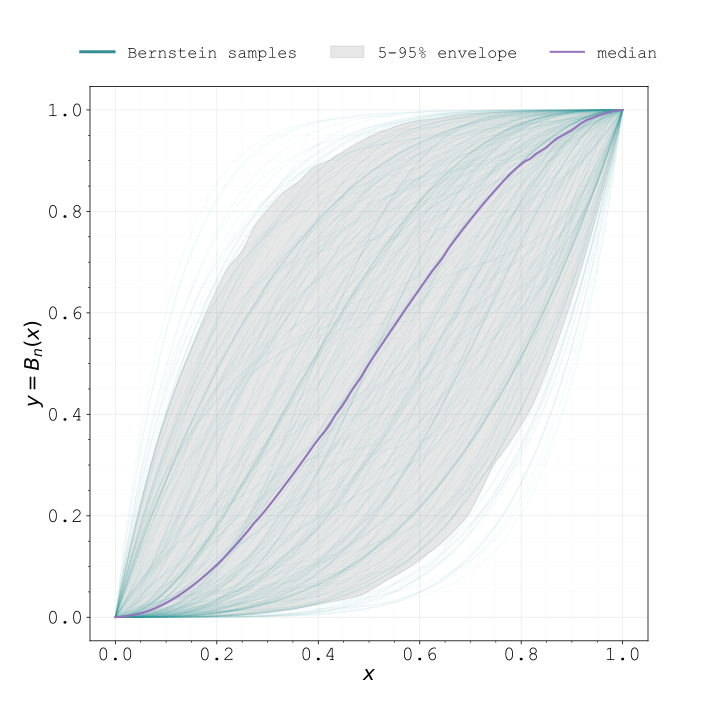
\includegraphics[width=0.37\textwidth]{img/bernstein}
	\caption{Zufällige Bernsteinpolynome fungieren als verschiedene kumulative Verteilungsfunktionen für die probabilistischen opaken Prädikate.} %mit $k=0$ und $a=1$
	\label{fig:bernstein}
\end{wrapfigure}

%Dadurch, dass $F$ monoton steigend ist, lässt sich $F$ als sortierte Liste an $y$-Werten betrachten. Das Inverse der kumulativen Verteilungsfunktion lässt sich folglich  über eine Binärsuche effizient in $\mathcal{O}(\log(n))$ wie folgt berechnen:
%Die Berechnung des Inversen der kumulativen Verteilungsfunktion geschieht über Binärsuche folgendermaßen:
Das Inverse der kumulativen Verteilungsfunktion lässt sich effizient über das Newton-Raphson-Verfahren in $O(k)$ berechnen, wobei $k$ die Anzahl an Iterationen festlegt. Aufgrund des quadratischen Konvergenzverhaltens des Verfahrens genügen für $64$-Bit Gleitkommazahlen praktisch $k=6$ Iterationen: Gemäß der IEEE 754 Norm haben $64$-Bit Gleitkommazahlen eine $52$-Bit Mantisse. Durch das Konvergenzverhalten verdoppelt sich die Anzahl korrekter Bits mit jeder Iteration. Ist anfänglich $1$ Bit korrekt erraten, so braucht es $6$ Iterationen, um alle $2^6=64>53$ Bits der Mantisse korrekt zu bestimmen. Um Sicherheitsgarantien zu liefern wurde der Algorithmus mit $k=12$ implementiert, um bei schlechten anfänglichen Schätzungen und ungünstigen Bernsteinpolynomen dennoch garantiert  das Inverse der kumulativen Verteilungsfunktion korrekt zu bestimmen. Die zusätzlichen Laufzeitkosten hierdurch sind minimal. \textcolor{red}{TODO: Auf chaotisches Verhalten/Divergenz eingehen!}
\begin{algorithm}[!h] 
	\caption{Berechnung der inversen kumulativen Verteilungsfunktion über das Newton-Raphson-Verfahren }
	\label{alg:invCumSum}
	\begin{algorithmic}[1]
		\Require $\Var{C}$ (Bernstein coefficients), $\Var{HShift}, \Var{HStretch}$ (Horizontal shift/stretch), $\Var{Precision}$ (determines precision of Bernstein evaluation) %\textbf{as hardcoded constants}
		\Function{SampleBernsteinInverse}{$\Var{U} \in [0, 1]$}
		\State $\Var{Estimate} \gets \Var{HShift} + \frac{0.5}{\Var{HStretch}}$ \Comment{Start guess at center of domain.}
		
		\For{$i \gets 0$ \textbf{to} $\Var{Precision}$}
			\State $\Var{t} \gets \Var{HStretch} \cdot (\Var{Estimate} - \Var{HShift})$ \Comment{Transformed $\Var{Estimate}$.}
			\State $\Var{y} \gets 0.0$ \Comment{Accumulator for $B(t)$.}
			\State $\Var{y'} \gets 0.0$ \Comment{Accumulator for $B'(t)$.}
			
			\For{$\Var{k} \gets 0$ \textbf{to} $\Var{Degree}$} \Comment{Evaluate CDF $B(t)$}
			\State $\Var{b_{k}} \gets \binom{n}{k} \cdot t^k \cdot (1-t)^{n-k}$ 
			\State $\Var{y} \gets \Var{y} + \Var{C}[k] \cdot \Var{b_{k}}$
			\EndFor
			
			\For{$\Var{k} \gets 0$ \textbf{to} $\Var{Degree}-1$} \Comment{Evaluate PDF.}
			\State $\Var{b'_{k}} \gets \binom{n-1}{k} \cdot t^k \cdot (1-t)^{n-1-k}$ 
			\State $\Var{y'} \gets \Var{y'} + \Var{C'}[k] \cdot \Var{b'_{k}}$
			\EndFor
			
			\State $\Var{OffsetY} \gets \Var{y} - \Var{U}$
			\State $\Var{Slope} \gets \Var{y'} \cdot \Var{HStretch}$ \Comment{Apply chain rule: $\frac{dy}{dx} = \frac{dy}{dt} \cdot \frac{dt}{dx}$.}
			
			\State $\Var{Estimate} \gets \Var{Estimate} - \frac{\Var{OffsetY}}{\Var{Slope}}$ \Comment{Newton Step.}
		\EndFor
		
		\State \Return $\Var{Estimate}$
		\EndFunction
	\end{algorithmic}
\end{algorithm}

\section{Implementierung}
\subsection{Entscheidungen}
Zur Implementierung wurden drei Ansätze erwogen: die Entwicklung eines Bin2Bin-Obfuskators\footnote{Direkte Manipulation von Assembler-Anweisungen existierender Programme.}, die Implementierung in Form eines LLVM-Passes \cite{LLVM, LLVMProject}\footnote{Nutzung des LLVM-Projekts, um einen sog. \emph{Compiler-Pass} zu schreiben.} sowie die Quellcodemanipulation\footnote{durch z.B. C-Makros und das Einfügen von inline Assembler-Ausschnitten}
Es wurde eine Entscheidung für einen LLVM-Pass getroffen aufgrund folgender Vorteile:

\begin{enumerate}[]
    \item \textbf{Abstraktion und Portabilität:} LLVM entkoppelt durch eine abstrakte Zwischensprache (\emph{Intermediate Representation}) von Architektur-/Betriebssystemdetails. Viele \emph{low-level} Aufgaben (z.B. \emph{Relocations}, Einfügen von Assembler-Anweisungen etc.) werden übernommen.
    \item \textbf{Optimierung:} Die LLVM-Toolchain enthält etablierte Optimierungs-Pässe und profitiert fortlaufend von der Arbeit zahlreicher Beiträgender. Dies ermöglicht eine nahezu optimale Kompilation obfuskierter Programme, welche sich als nützlich und sogar erforderlich in vielen Anweundungssituationen erweist (z.B. \emph{Embedded Systems}, IoT, Echtzeitsysteme etc.).
    \item \textbf{Entwicklungsaufwand:} Bin2Bin-Obfuskatoren und umfangreiche Quellcodemanipulation erfordern viel manuellen Aufwand und sind fehlerhaftig. Ein LLVM-Pass ermöglicht den reinen Fokus auf die Obfuskationslogik.
\end{enumerate}

\begin{figure}[h]
    \centering
    \includegraphics[width=0.8\linewidth]{img/llvm-pass}
    \caption{Schematische Darstellung eines LLVM-basierten Build-Prozesses mit optionalem Obfuskator-Pass.}
    \label{fig:llvm-pass}
\end{figure}

Ein LLVM-Pass bietet in diesem Fall das beste Kompromissverhältnis zwischen \emph{low-level} Kontrolle, Laufzeiteffizienz, einer \emph{high-level} Portabilität sowie geringem Entwicklungsaufwand.

Die Implementierung, Beispiele und Experimente sind unter \url{https://github.com/sariaki/JuFo-2026} zu finden. Da in der Implementierung alle Zufahlszahlen vom selben PRNG generiert werden, kann der anfängliche Startwert (\emph{Seed}) als Schlüssel für die Obfuskation betrachtet werden.
%\textcolor{red}{TODO: Inspiration von ogisoSoftwareObfuscationTheoretical2003 nehmen!}

%\subsection{Generierung von Pseudozufallsvariablen} \label{sec:pseudoZufall}
%\textcolor{red}{TODO: Das hier kürzen/verschieben/löschen}
%%Damit der vorgestellte Ansatz funktionieren kann, bedarf er einer gleichverteilten (Pseudo-)Zufallszahl, welche auf dem Einheitsintervall liegt und zugleich als unbestimmte symbolische Variable von symbolischen Ausführungsengines betrachtet wird.
%Das Ziel dieses Abschnittes ist es, gleichverteilte Pseudozufallszahlen im Einheitsintervall zu generieren, sodass symbolische Ausführungsengines diese als symbolische Variablen behandeln, ohne ihnen einen konkreten Wert zuweisen zu können. Folgende Methoden existieren hierfür:
%%Hierfür werden die Parameter der obfuskierten Funktionen verwendet. Die Idee hierhinter ist, dass um diese zu bestimmen, ...
%%Hat die zu obfuskierende Funktion kein Parameter, so kann ein Pseudoparameter hinzugefügt werden. 
%%Um zu garantieren, dass die generierte Pseudozufallszahl im Einheitsintervall liegt, existieren mehrere Methoden. Es wurde sich für die einfachste Entschieden. Hier wird der erste Parameter als $64$-Bit Gleitkommazahl betrachtet und durch dessen maximalen Wert geteilt.
%
%\paragraph{Explizite Quellen (Betriebssystem-APIs, Hardware)}
%CPUs und Betriebssysteme bieten mehrere Methoden, welche sich für die Zufallszahlgenerierung eignen (z.B. \texttt{rdtsc}, \texttt{rand() oder \texttt{time()}}). 
%In beiden Fällen sind die genutzten Quellen leicht erkennbar. Dies erleichtert für Angreifer die Suche nach probabilistischen opaken Prädikaten und folglich auch ihre Tarnung.
%
%\paragraph{Parameter-Sampling}
%In der Praxis versuchen Angreifer nie, ganze Programme symbolisch auszuführen sondern immer nur einzelne Funktionen. Beim Parameter-Sampling wird dies genutzt: Die Parameterwerte einer Funktion lassen sich alleine betrachtet nicht bestimmen, sie werden vom symbolischen Ausführungsengine als symbolische Variablen behandelt.
%
%Dies bietet den Vorteil, dass die opaken Prädikate gut getarnt sind - ein Parameterzugriff ist schließlich normales Verhalten in jedem Programm. Problematisch ist dabei, dass manche Parameter bei jedem Aufruf innerhalb eines Programms gleich bleiben und leicht zu bestimmen sind. Die Lösung probabilistischer opaker Prädikate durch einen Angreifer erfordert demnach nur eine Bestimmung des konstanten Parameterwerts.
%
%\paragraph{Race Conditions}
%Das gleichzeitige Überschreiben einer Variable mit verschiedenen Werten durch zwei Threads \cite{colesaRandomRace}  \textcolor{red}{TODO...} \\
%
%Aufgrund ihrer Geschwindigkeit, Unauffälligkeit sowie Einfachheit wurde die Pseudozufallszahlgenerierung über Parameter-Sampling implementiert.
%
%\subsection{Füllcode}
%\textcolor{red}{Ohne gut getarnten Füllcode ist eine Erkennung des unwahrscheinlichen Prädikats trivial. Der Pfad, welcher die plausibelsten Anweisungen enthält ist der Richtige, die Qualität des opaken Prädikats ändert daran nichts. Hierfür wurde die Methode von \cite{} implementiert.}

\subsection{Fallbeispiel}
\begin{figure}[!h]
	\centering 
	
	\begin{minipage}[c]{0.36\textwidth}
		\begin{subfigure}[b]{\linewidth}
			\begin{lstlisting}[style=customc_compact, captionpos=b, language=bash]	
#!/bin/bash

OPT_LVL=O0
FILENAME="hello_world"
PASS_PLUGIN_DIR="Obfuscator.so"
PROB=50

clang -$OPT_LVL \
	-fpass-plugin=$PASS_PLUGIN_DIR \
	-Xclang -load $PASS_PLUGIN_DIR \
	-mllvm -pop-probability=$PROB \
	${FILENAME}.c \
	-o $FILENAME\end{lstlisting}
			\caption{Bash-Skript zur Ausführung der implementierten Obfuskation auf C(++) Quellcode.}
		\end{subfigure}
		
		\vspace{1em}
		
		\begin{subfigure}[b]{\linewidth}
			\begin{lstlisting}[style=customc_compact, captionpos=b]	
__attribute__(annotate("POP"))
void foo(int x)
{
	printf("foo %i\n", x);
}			\end{lstlisting}
			\caption{Eine einfache zu obfuskierende Funktion.}
			\label{fig:toObf}
		\end{subfigure}
	\end{minipage}
	\hfill
	\begin{minipage}[c]{0.6\textwidth}
		\begin{subfigure}[c]{\linewidth}
			\begin{lstlisting}[style=customc_compact, captionpos=b, firstnumber=1]
void __cdecl foo(int x)
{
	double v1;
	double v2;
	double v3;
	int i;
	
	v3 = 20.7517909733016;
	for ( i = 0; i != 16; ++i )
	{
		v1 = (v3 - 20.70639451264049) * 11.01407450533519;
		v2 = v3
		- (0.0 * ((1.0 - v1) * (1.0 - v1) * (1.0 - v1))
		+ 0.0
		+ 0.3788140306973082 * v1 * ((1.0 - v1) * (1.0 - v1))
		+ 1.326401583206529 * (v1 * v1) * (1.0 - v1)
		+ v1 * v1 * v1
		- (double)x * COERCE_DOUBLE(0x4000000000000LL))
		/ ((0.3788140306973082 * ((1.0 - v1) * (1.0 - v1))
		+ 0.0
		+ 1.895175105018441 * v1 * (1.0 - v1)
		+ 1.673598416793471 * (v1 * v1))
		* 11.01407450533519);
		v3 = v2;
	}
	if ( v2 >= 19.80279674504742 )
	{
		// Junkcode
		return; // This Basic Block is never reached.
	}
	printf("foo %i\n", x); // This Basic Block will always be executed.
}			\end{lstlisting}
			\caption{Dieselbe Funktion aber mit PoP (Bernsteinpolynomgrad $n=3 $) obfuskiert. Pseudo-C wurde aus der Dekompilation von IDA entnommen.\textcolor{red}{TODO: update mit neuer Version}}
			\label{fig:doneObf}
		\end{subfigure}
	\end{minipage}
\end{figure}

\section{Evaluierung}
\subsection{Vorgehen} \label{sec:kriterien}
Für die Evaluierung wird gemäß der weitverbreiteten Kriterien von Collberg et al. \cite{collbergATaxonomyOfObfuscatingTransformations} vorgegangen\label{par:metriken}:

\begin{center}
    \begin{tabular}{c|l}
    	\textbf{Kriterium} & \textbf{Beschreibung} \\
    	\hline
    	Stärke & Wie unverständlich ist die Obfuskation für einen Angreifer? \\
    	\hline
    	Resilienz & Wie schwer ist eine (automatisierte) Deobfuskation? \\
    	\hline
    	Kosten & Wie sehr erhöht die Obfuskation die Laufzeitkosten? \\
    	\hline
    	Tarnung & Wie auffällig ist die Obfuskation? %Wie leicht lässt sich ein obfuskiertes Programm als solches erkennen? \\
    \end{tabular}
\end{center}

Die Obfuskationsmethode wurde dabei auf Programme aus \cite{banescuCodeObfuscationSymbolic2016}\footnote{\url{https://github.com/tum-i4/obfuscation-benchmarks}}, auf mehrere Verschlüsselungs-/Hashverfahren (AES, DES, MD5, RC4 \& SHA1.) von \cite{ollivierHowKillSymbolic2019a} sowie auf die GNU Core Utilities angewandt. Die Programme wurden gewählt, um repräsentativ typische Szenarien abzubilden, in denen z.B. kryptographische Algorithmen zum Schutz geistigen Eigentums eingesetzt werden \cite{schloegelTechnicalReportHardening2022}.

Alle Programme wurden mit clang 18.1.3 und Optimierungslevel \texttt{-O3} kompilliert.

Folgende Angriffsmethoden werden betrachtet: 
\begin{itemize}
	\item Symbolische Ausführung mit Angr \cite{shoshitaishvili2016state} (v.9.2.189), Triton \cite{SSTIC2015-Saudel-Salwan} (v.1.0.0rc4) und Miasm \cite{desclaux2018miasm} (v.0.1.5)

	\item Programmsynthese mittels Syntia \cite{blazytkoSyntiaSynthesizingSemanticsa} (commit 3602893) 

	\item dynamische Analyse über mehrfache Ausführung obfuskierter Programme wie in \cite{zobernigWhenAreOpaque2019} beschrieben

	\item Pattern Matching
\end{itemize}
Alle Experimente wurden mit Ubuntu 24.04.3 LTS mit Kernel Version 5.16, einer Intel\textregistered \;Core\texttrademark \;i7-10700F CPU und $16$Gb DDR4 RAM ausgeführt.

\subsection{Evaluierung}

\subsubsection{Kosten}

\paragraph{Programmgröße}
\paragraph{Geschwindigkeit}
\paragraph{Arbeitsspeicheraufwand}
%\paragraph{Kompilationszeit}

\subsubsection{Tarnung}

\paragraph{Opcode Verteilung}
\paragraph{Entropie}

\subsubsection{Resilienz}

\subsubsection{Stärke} \label{sec:stärke}

\paragraph{Komplexität}
\paragraph{Menschliche Analyse}

\subsection{Vergleich mit existierenden Obfuskationsmethoden}

%\subsection{Praktische Anwendung}

\section{Ergebnisdiskussion}
\section{Fazit und Ausblick} \label{sec:fazit}
\textcolor{red}{Verbesserung durch Anwendung anderer Obfuscationsmethoden (z.B. MBAs)} \\
\textcolor{red}{später: Anwendung auf Ausdrücke}

\newpage
\pagenumbering{Alph}

%\section*{Quellen- und Literaturverzeichnis}
\printbibliography[title=Literaturverzeichnis]
\addcontentsline{toc}{section}{Literaturverzeichnis}
\listoffigures
\addcontentsline{toc}{section}{Abbildungsverzeichnis}

\end{document}